\documentclass[11pt,a4paper,]{article}
\usepackage{lmodern}

\usepackage{amssymb,amsmath}
\usepackage{ifxetex,ifluatex}
\usepackage{fixltx2e} % provides \textsubscript
\ifnum 0\ifxetex 1\fi\ifluatex 1\fi=0 % if pdftex
  \usepackage[T1]{fontenc}
  \usepackage[utf8]{inputenc}
\else % if luatex or xelatex
  \usepackage{unicode-math}
  \defaultfontfeatures{Ligatures=TeX,Scale=MatchLowercase}
\fi
% use upquote if available, for straight quotes in verbatim environments
\IfFileExists{upquote.sty}{\usepackage{upquote}}{}
% use microtype if available
\IfFileExists{microtype.sty}{%
\usepackage[]{microtype}
\UseMicrotypeSet[protrusion]{basicmath} % disable protrusion for tt fonts
}{}
\PassOptionsToPackage{hyphens}{url} % url is loaded by hyperref
\usepackage[unicode=true]{hyperref}
\hypersetup{
            pdftitle={Crime in Minneapolis},
            pdfborder={0 0 0},
            breaklinks=true}
\urlstyle{same}  % don't use monospace font for urls
\usepackage{geometry}
\geometry{a4paper, centering, text={16cm,24cm}}
\usepackage[style=authoryear-comp,]{biblatex}
\addbibresource{references.bib}
\usepackage{color}
\usepackage{fancyvrb}
\newcommand{\VerbBar}{|}
\newcommand{\VERB}{\Verb[commandchars=\\\{\}]}
\DefineVerbatimEnvironment{Highlighting}{Verbatim}{commandchars=\\\{\}}
% Add ',fontsize=\small' for more characters per line
\usepackage{framed}
\definecolor{shadecolor}{RGB}{248,248,248}
\newenvironment{Shaded}{\begin{snugshade}}{\end{snugshade}}
\newcommand{\AlertTok}[1]{\textcolor[rgb]{0.94,0.16,0.16}{#1}}
\newcommand{\AnnotationTok}[1]{\textcolor[rgb]{0.56,0.35,0.01}{\textbf{\textit{#1}}}}
\newcommand{\AttributeTok}[1]{\textcolor[rgb]{0.77,0.63,0.00}{#1}}
\newcommand{\BaseNTok}[1]{\textcolor[rgb]{0.00,0.00,0.81}{#1}}
\newcommand{\BuiltInTok}[1]{#1}
\newcommand{\CharTok}[1]{\textcolor[rgb]{0.31,0.60,0.02}{#1}}
\newcommand{\CommentTok}[1]{\textcolor[rgb]{0.56,0.35,0.01}{\textit{#1}}}
\newcommand{\CommentVarTok}[1]{\textcolor[rgb]{0.56,0.35,0.01}{\textbf{\textit{#1}}}}
\newcommand{\ConstantTok}[1]{\textcolor[rgb]{0.00,0.00,0.00}{#1}}
\newcommand{\ControlFlowTok}[1]{\textcolor[rgb]{0.13,0.29,0.53}{\textbf{#1}}}
\newcommand{\DataTypeTok}[1]{\textcolor[rgb]{0.13,0.29,0.53}{#1}}
\newcommand{\DecValTok}[1]{\textcolor[rgb]{0.00,0.00,0.81}{#1}}
\newcommand{\DocumentationTok}[1]{\textcolor[rgb]{0.56,0.35,0.01}{\textbf{\textit{#1}}}}
\newcommand{\ErrorTok}[1]{\textcolor[rgb]{0.64,0.00,0.00}{\textbf{#1}}}
\newcommand{\ExtensionTok}[1]{#1}
\newcommand{\FloatTok}[1]{\textcolor[rgb]{0.00,0.00,0.81}{#1}}
\newcommand{\FunctionTok}[1]{\textcolor[rgb]{0.00,0.00,0.00}{#1}}
\newcommand{\ImportTok}[1]{#1}
\newcommand{\InformationTok}[1]{\textcolor[rgb]{0.56,0.35,0.01}{\textbf{\textit{#1}}}}
\newcommand{\KeywordTok}[1]{\textcolor[rgb]{0.13,0.29,0.53}{\textbf{#1}}}
\newcommand{\NormalTok}[1]{#1}
\newcommand{\OperatorTok}[1]{\textcolor[rgb]{0.81,0.36,0.00}{\textbf{#1}}}
\newcommand{\OtherTok}[1]{\textcolor[rgb]{0.56,0.35,0.01}{#1}}
\newcommand{\PreprocessorTok}[1]{\textcolor[rgb]{0.56,0.35,0.01}{\textit{#1}}}
\newcommand{\RegionMarkerTok}[1]{#1}
\newcommand{\SpecialCharTok}[1]{\textcolor[rgb]{0.00,0.00,0.00}{#1}}
\newcommand{\SpecialStringTok}[1]{\textcolor[rgb]{0.31,0.60,0.02}{#1}}
\newcommand{\StringTok}[1]{\textcolor[rgb]{0.31,0.60,0.02}{#1}}
\newcommand{\VariableTok}[1]{\textcolor[rgb]{0.00,0.00,0.00}{#1}}
\newcommand{\VerbatimStringTok}[1]{\textcolor[rgb]{0.31,0.60,0.02}{#1}}
\newcommand{\WarningTok}[1]{\textcolor[rgb]{0.56,0.35,0.01}{\textbf{\textit{#1}}}}
\usepackage{longtable,booktabs}
% Fix footnotes in tables (requires footnote package)
\IfFileExists{footnote.sty}{\usepackage{footnote}\makesavenoteenv{long table}}{}
\usepackage{graphicx,grffile}
\makeatletter
\def\maxwidth{\ifdim\Gin@nat@width>\linewidth\linewidth\else\Gin@nat@width\fi}
\def\maxheight{\ifdim\Gin@nat@height>\textheight\textheight\else\Gin@nat@height\fi}
\makeatother
% Scale images if necessary, so that they will not overflow the page
% margins by default, and it is still possible to overwrite the defaults
% using explicit options in \includegraphics[width, height, ...]{}
\setkeys{Gin}{width=\maxwidth,height=\maxheight,keepaspectratio}
\IfFileExists{parskip.sty}{%
\usepackage{parskip}
}{% else
\setlength{\parindent}{0pt}
\setlength{\parskip}{6pt plus 2pt minus 1pt}
}
\setlength{\emergencystretch}{3em}  % prevent overfull lines
\providecommand{\tightlist}{%
  \setlength{\itemsep}{0pt}\setlength{\parskip}{0pt}}
\setcounter{secnumdepth}{5}

% set default figure placement to htbp
\makeatletter
\def\fps@figure{htbp}
\makeatother


\title{Crime in Minneapolis}

%% MONASH STUFF

%% CAPTIONS
\RequirePackage{caption}
\DeclareCaptionStyle{italic}[justification=centering]
 {labelfont={bf},textfont={it},labelsep=colon}
\captionsetup[figure]{style=italic,format=hang,singlelinecheck=true}
\captionsetup[table]{style=italic,format=hang,singlelinecheck=true}


%% FONT
\RequirePackage{bera}
\RequirePackage[charter,expert,sfscaled]{mathdesign}
\RequirePackage{fontawesome}

%% HEADERS AND FOOTERS
\RequirePackage{fancyhdr}
\pagestyle{fancy}
\rfoot{\Large\sffamily\raisebox{-0.1cm}{\textbf{\thepage}}}
\makeatletter
\lhead{\textsf{\expandafter{\@title}}}
\makeatother
\rhead{}
\cfoot{}
\setlength{\headheight}{15pt}
\renewcommand{\headrulewidth}{0.4pt}
\renewcommand{\footrulewidth}{0.4pt}
\fancypagestyle{plain}{%
\fancyhf{} % clear all header and footer fields
\fancyfoot[C]{\sffamily\thepage} % except the center
\renewcommand{\headrulewidth}{0pt}
\renewcommand{\footrulewidth}{0pt}}

%% MATHS
\RequirePackage{bm,amsmath}
\allowdisplaybreaks

%% GRAPHICS
\RequirePackage{graphicx}
\setcounter{topnumber}{2}
\setcounter{bottomnumber}{2}
\setcounter{totalnumber}{4}
\renewcommand{\topfraction}{0.85}
\renewcommand{\bottomfraction}{0.85}
\renewcommand{\textfraction}{0.15}
\renewcommand{\floatpagefraction}{0.8}


%\RequirePackage[section]{placeins}

%% SECTION TITLES


%% SECTION TITLES (NEW: Changing sections and subsections color)  
\RequirePackage[compact,sf,bf]{titlesec}
\titleformat*{\section}{\Large\sf\bfseries\color[rgb]{0.8, 0.7, 0.1 }}
\titleformat*{\subsection}{\large\sf\bfseries\color[rgb]{0.8, 0.7, 0.1 }}
\titleformat*{\subsubsection}{\sf\bfseries\color[rgb]{0.8, 0.7, 0.1 }}
\titlespacing{\section}{0pt}{2ex}{.5ex}
\titlespacing{\subsection}{0pt}{1.5ex}{0ex}
\titlespacing{\subsubsection}{0pt}{.5ex}{0ex}


%% TITLE PAGE
\def\Date{\number\day}
\def\Month{\ifcase\month\or
 January\or February\or March\or April\or May\or June\or
 July\or August\or September\or October\or November\or December\fi}
\def\Year{\number\year}

%% LINE AND PAGE BREAKING
\sloppy
\clubpenalty = 10000
\widowpenalty = 10000
\brokenpenalty = 10000
\RequirePackage{microtype}

%% PARAGRAPH BREAKS
\setlength{\parskip}{1.4ex}
\setlength{\parindent}{0em}

%% HYPERLINKS
\RequirePackage{xcolor} % Needed for links
\definecolor{darkblue}{rgb}{0,0,.6}
\RequirePackage{url}

\makeatletter
\@ifpackageloaded{hyperref}{}{\RequirePackage{hyperref}}
\makeatother
\hypersetup{
     citecolor=0 0 0,
     breaklinks=true,
     bookmarksopen=true,
     bookmarksnumbered=true,
     linkcolor=darkblue,
     urlcolor=blue,
     citecolor=darkblue,
     colorlinks=true}

\usepackage[showonlyrefs]{mathtools}
\usepackage[no-weekday]{eukdate}

%% BIBLIOGRAPHY   %------------------------------------------------------------------------------------------------

\makeatletter
\@ifpackageloaded{biblatex}{}{\usepackage[style=authoryear-comp, backend=biber, natbib=true]{biblatex}}
\makeatother
\ExecuteBibliographyOptions{bibencoding=utf8,minnames=1,maxnames=3, maxbibnames=99,dashed=false,terseinits=true,giveninits=true,uniquename=false,uniquelist=false,doi=false, isbn=false,url=true,sortcites=false}

\DeclareFieldFormat{url}{\texttt{\url{#1}}}
\DeclareFieldFormat[article]{pages}{#1}
\DeclareFieldFormat[inproceedings]{pages}{\lowercase{pp.}#1}
\DeclareFieldFormat[incollection]{pages}{\lowercase{pp.}#1}
\DeclareFieldFormat[article]{volume}{\mkbibbold{#1}}
\DeclareFieldFormat[article]{number}{\mkbibparens{#1}}
\DeclareFieldFormat[article]{title}{\MakeCapital{#1}}
\DeclareFieldFormat[article]{url}{}
%\DeclareFieldFormat[book]{url}{}
%\DeclareFieldFormat[inbook]{url}{}
%\DeclareFieldFormat[incollection]{url}{}
%\DeclareFieldFormat[inproceedings]{url}{}
\DeclareFieldFormat[inproceedings]{title}{#1}
\DeclareFieldFormat{shorthandwidth}{#1}
%\DeclareFieldFormat{extrayear}{}
% No dot before number of articles
\usepackage{xpatch}
\xpatchbibmacro{volume+number+eid}{\setunit*{\adddot}}{}{}{}
% Remove In: for an article.
\renewbibmacro{in:}{%
  \ifentrytype{article}{}{%
  \printtext{\bibstring{in}\intitlepunct}}}

\AtEveryBibitem{\clearfield{month}}
\AtEveryCitekey{\clearfield{month}}

\makeatletter
\DeclareDelimFormat[cbx@textcite]{nameyeardelim}{\addspace}
\makeatother

\author{\sf\Large\textbf{ Lulu Pi}\\ {\sf\large XXX\\[0.5cm]} \sf\Large\textbf{ Emily Sheehan}\\ {\sf\large BComm\\[0.5cm]} \sf\Large\textbf{ Brenwin Ang}\\ {\sf\large XXX\\[0.5cm]} \sf\Large\textbf{ Chengzhi Ye}\\ {\sf\large XXX\\[0.5cm]}}

\date{\sf\Date~\Month~\Year}
\makeatletter
\lfoot{\sf Pi, Sheehan, Ang, Ye: \@date}
\makeatother


%%%% PAGE STYLE FOR FRONT PAGE OF REPORTS    %----------------------------------------------------------------------------------------

\makeatletter
\def\organization#1{\gdef\@organization{#1}}
\def\telephone#1{\gdef\@telephone{#1}}
\def\email#1{\gdef\@email{#1}}
\makeatother
  \organization{Monash University}

  \def\name{Faculty of \newline Business \&\newline Economics}

  \telephone{(03) 9905 2478}

  \email{questions@company.com}                 %NEW: New email addresss ---------------------------------------

\def\webaddress{\url{http://company.com/stats/consulting/}} %NEW: URl  ------------------------------------------
\def\abn{12 377 614 630}                                    % NEW: ABN -------------------------------------------  
\def\logo{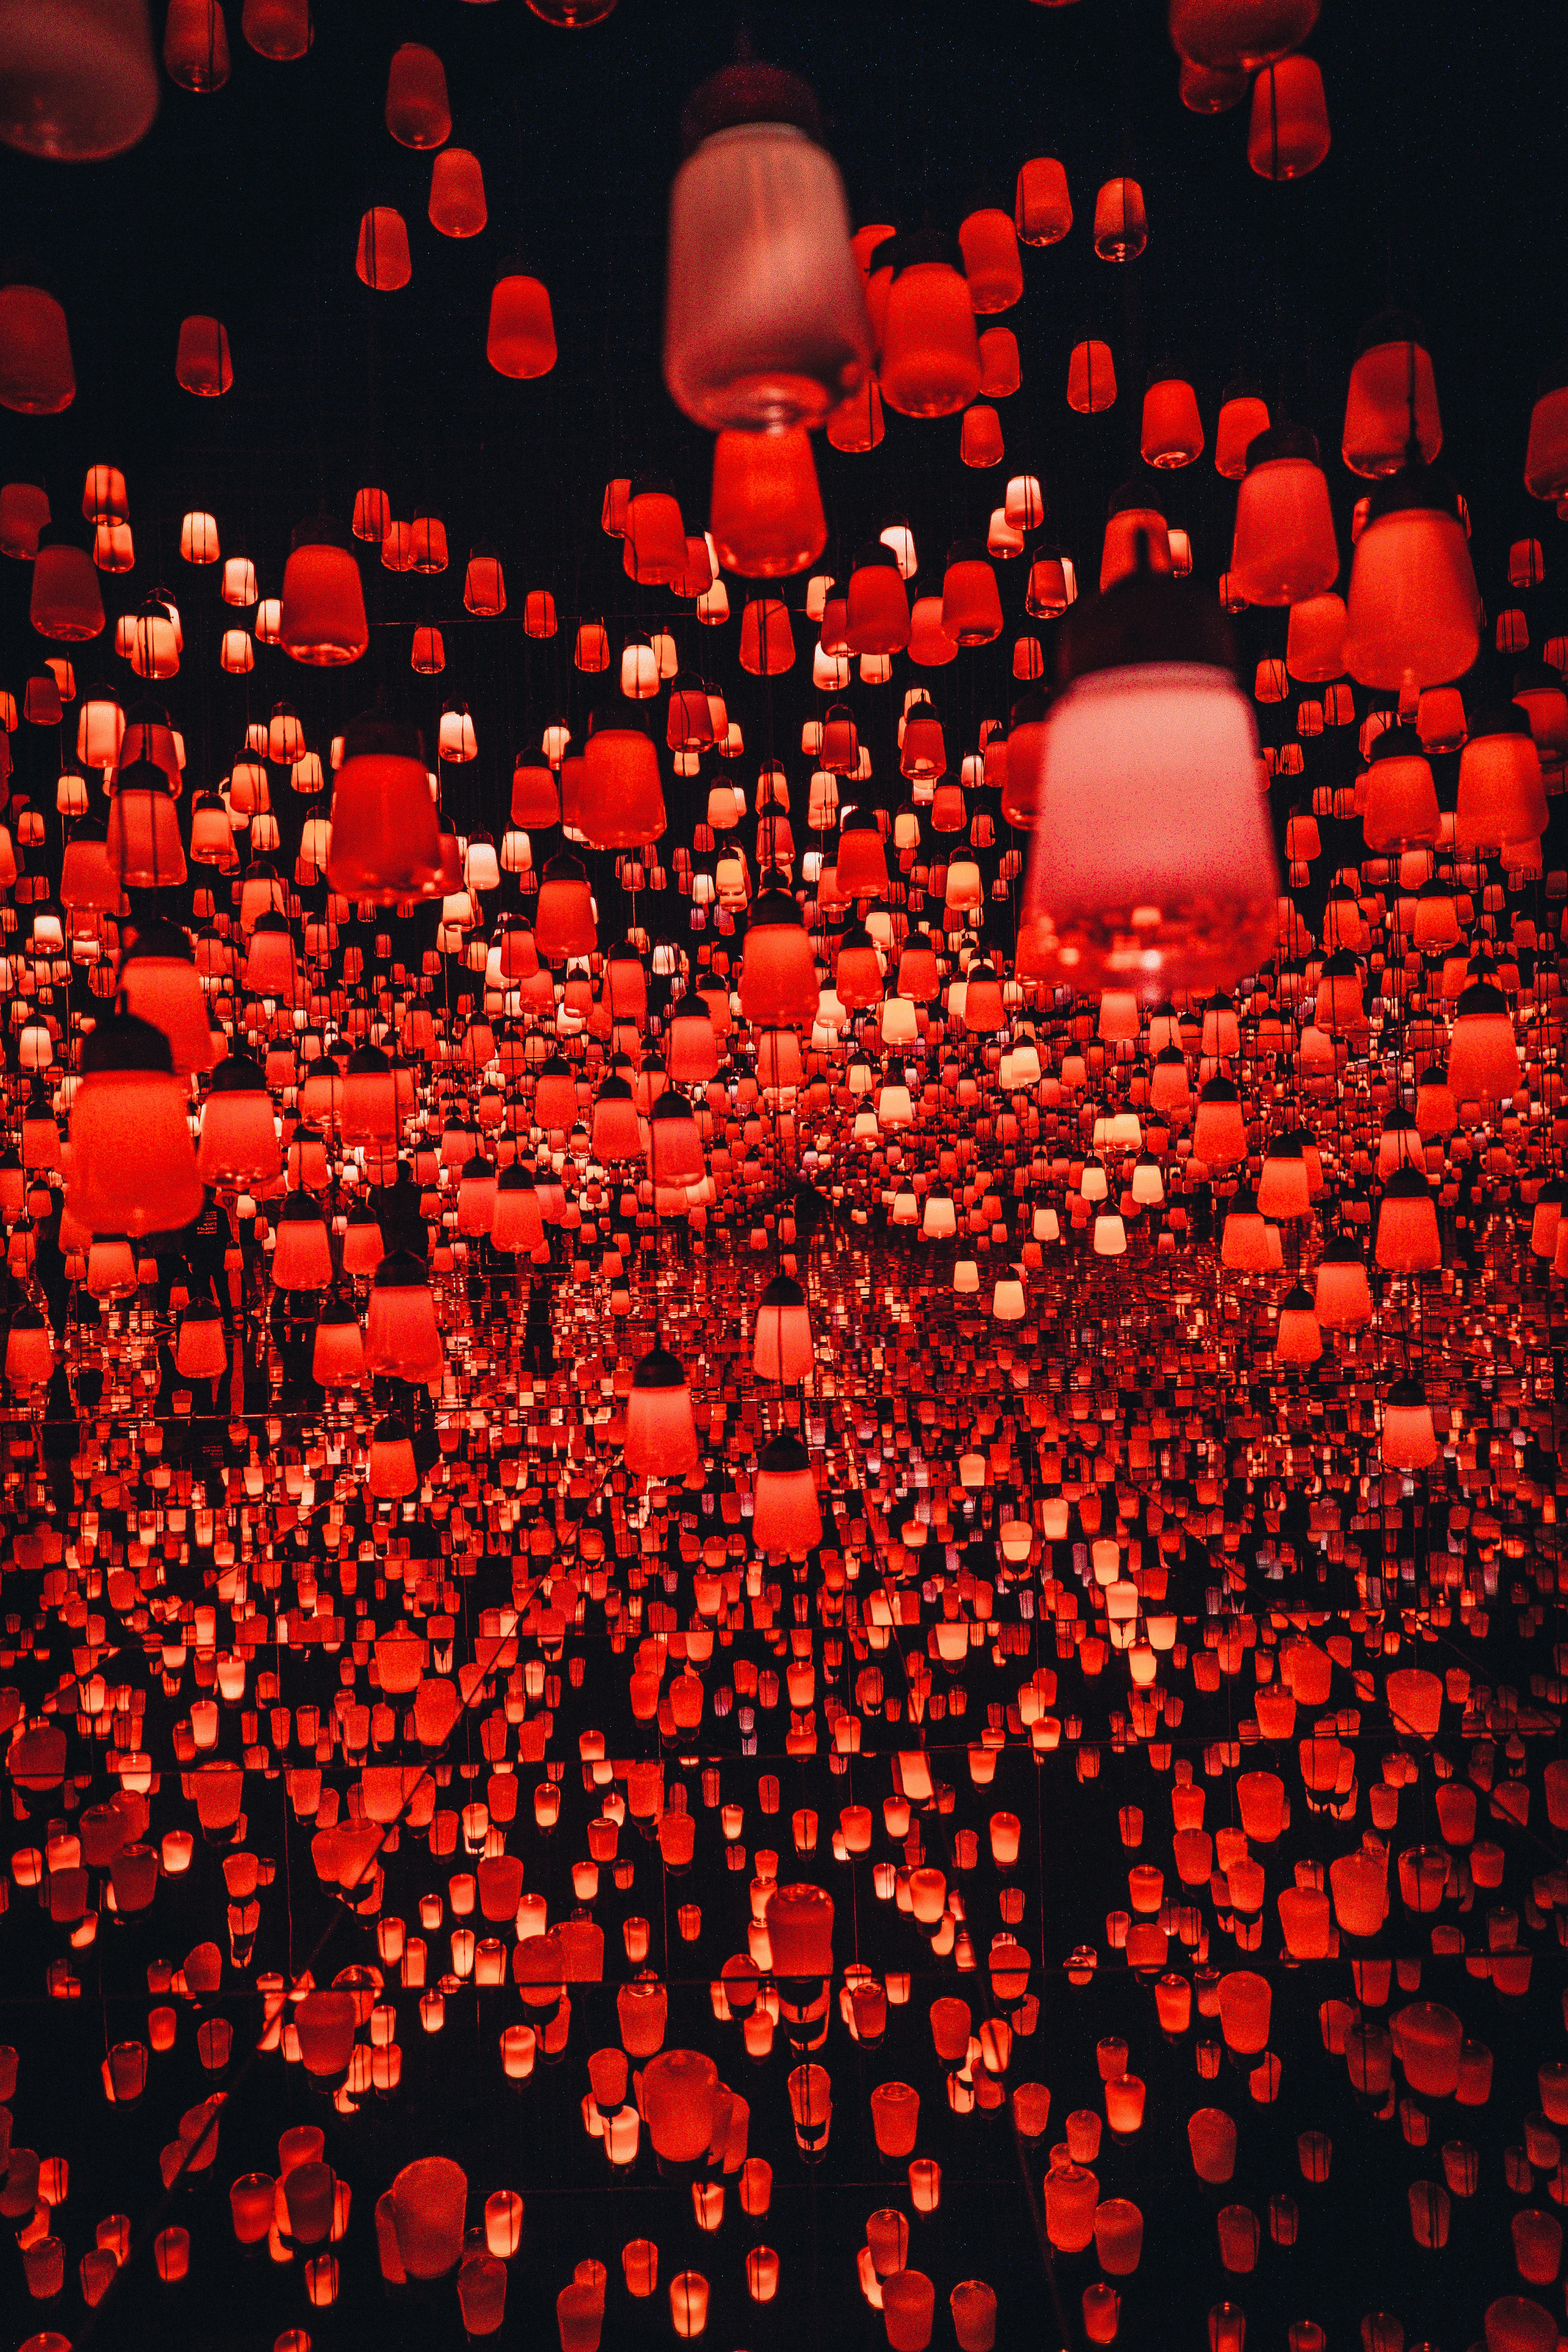
\includegraphics[width=6cm]{logo}}  %NEW: Changing logo
\def\extraspace{\vspace*{1.6cm}}
\makeatletter
\def\contactdetails{\faicon{phone} & \@telephone \\
                    \faicon{envelope} & \@email}
\makeatother

%%%% FRONT PAGE OF REPORTS

\def\reporttype{Report for}

\long\def\front#1#2#3{
\newpage
\begin{singlespacing}
\thispagestyle{empty}
\vspace*{-1.4cm}
\hspace*{-1.4cm}
\hbox to 16cm{
  \hbox to 6.5cm{\vbox to 14cm{\vbox to 25cm{
    \logo
    \vfill
    \parbox{6.3cm}{\raggedright
      \sf\color[rgb]{0, 0.29, 0.55}    % NEW color -company info------------------------------------------------------------------------------------
      {\large\textbf{\name}}\par
      \vspace{.7cm}
      \tabcolsep=0.12cm\sf\small
      \begin{tabular}{@{}ll@{}}\contactdetails
      \end{tabular}
      \vspace*{0.3cm}\par
      ABN: \abn\par
    }
  }\vss}\hss}
  \hspace*{0.2cm}
  \hbox to 1cm{\vbox to 14cm{\rule{4pt}{26.8cm}\vss}\hss\hfill}  %NEW: Thicker vertical line -----------------------------------------------------
  \hbox to 10cm{\vbox to 14cm{\vbox to 25cm{   
      \vspace*{3cm}\sf\raggedright
      \parbox{11cm}{\sf\raggedright\baselineskip=1.2cm
         \fontsize{24.88}{30}\color[rgb]{0, 0.29, 0.55}\sf\textbf{#1}}   % NEW: title color blue ----------------------------------------------
      \par
      \vfill
      \large
      \vbox{\parskip=0.8cm #2}\par
      \vspace*{2cm}\par
      \reporttype\\[0.3cm]
      \hbox{#3}%\\[2cm]\
      \vspace*{1cm}
      {\large\sf\textbf{\Date~\Month~\Year}}
   }\vss}
  }}
\end{singlespacing}
\newpage
}

\makeatletter
\def\titlepage{\front{\expandafter{\@title}}{\@author}{\@organization}}
\makeatother

\usepackage{setspace}
\setstretch{1.5}

%% Any special functions or other packages can be loaded here.
\usepackage{booktabs}
\usepackage{longtable}
\usepackage{array}
\usepackage{multirow}
\usepackage{wrapfig}
\usepackage{float}
\usepackage{colortbl}
\usepackage{pdflscape}
\usepackage{tabu}
\usepackage{threeparttable}
\usepackage{threeparttablex}
\usepackage[normalem]{ulem}
\usepackage{makecell}
\usepackage{xcolor}


\begin{document}           % Begining of document body -----------------------------------------------
\titlepage

{
\setcounter{tocdepth}{2}
\tableofcontents
}
Analysis of Crime in Minneapolis:

\begin{itemize}
\tightlist
\item
  What types of crimes are most common?
\item
  What crime is committed by each race? Are they proportionate?
\item
  What are the most common force types?
\item
  Which months of the year have the most criminal records?
\item
  Which day of the week has the most crimes or forces used by police?
\item
  Which area has the most crime?
\item
  Is it the same police committing each crime?
\end{itemize}

\begin{Shaded}
\begin{Highlighting}[]
\NormalTok{knitr}\OperatorTok{::}\NormalTok{opts_chunk}\OperatorTok{$}\KeywordTok{set}\NormalTok{(}\DataTypeTok{echo =} \OtherTok{FALSE}\NormalTok{, }
                      \DataTypeTok{cache=}\OtherTok{TRUE}\NormalTok{, }
                      \DataTypeTok{messages=}\OtherTok{FALSE}\NormalTok{,}
                      \DataTypeTok{warning=}\OtherTok{FALSE}\NormalTok{)}
\end{Highlighting}
\end{Shaded}

\begin{verbatim}
## Parsed with column specification:
## cols(
##   .default = col_character(),
##   X = col_double(),
##   Y = col_double(),
##   reportedTime = col_double(),
##   beginTime = col_double(),
##   centergbsid = col_double(),
##   centerLong = col_double(),
##   centerLat = col_double(),
##   centerX = col_double(),
##   centerY = col_double(),
##   OBJECTID = col_double()
## )
\end{verbatim}

\begin{verbatim}
## See spec(...) for full column specifications.
\end{verbatim}

\begin{verbatim}
## OGR data source with driver: ESRI Shapefile 
## Source: "/Users/emsheehan/Documents/UNI - POSTGRAD/COLLAB/ETC5513-Assignment-4/data/Police_Incidents_Last_2Years-shp/Police_Incidents_Last_2Years.shp", layer: "Police_Incidents_Last_2Years"
## with 43283 features
## It has 0 fields
\end{verbatim}

\begin{verbatim}
## Parsed with column specification:
## cols(
##   .default = col_character(),
##   X = col_double(),
##   Y = col_double(),
##   PoliceUseOfForceID = col_double(),
##   ForceReportNumber = col_double(),
##   SubjectRoleNumber = col_double(),
##   EventAge = col_double(),
##   TotalCityCallsForYear = col_double(),
##   TotalPrecinctCallsForYear = col_double(),
##   TotalNeighborhoodCallsForYear = col_double(),
##   CenterGBSID = col_double(),
##   CenterLatitude = col_double(),
##   CenterLongitude = col_double(),
##   CenterX = col_double(),
##   CenterY = col_double(),
##   OBJECTID = col_double()
## )
\end{verbatim}

\begin{verbatim}
## See spec(...) for full column specifications.
\end{verbatim}

\hypertarget{introduction}{%
\section{Introduction}\label{introduction}}

George Floyd was arrested and killed by Derek Chauvin, a U.S. police officer, on the 25th of May in Minneapolis, \textcite{BBC-News-2020}. Chauvin knelt on George Floyd's neck for eight minutes and 46 seconds as Floyd gasped for air. His abominable death has sparked outrage on police brutality across America.

For several years, African-Americans have been the subject of racial vilification. In a study by \textcite{Dottolo-2008} students were interviewed and asked about police harassment and crime. Close analysis revealed that the students had stereotyped the criminals to be poor African American men. Another study by \ldots{} revealed

This paper hopes to explore and understand crime in Minneapolis. Specifically, the areas where crime is most common, the ethnicity of those committing the crime, and the force used by police.

\hypertarget{data}{%
\section{Data}\label{data}}

To perform this analysis

\hypertarget{methodology}{%
\section{Methodology}\label{methodology}}

\hypertarget{analysis-on-neighborhoods-with-the-most-crimes}{%
\subsection{Analysis on neighborhoods with the most crimes}\label{analysis-on-neighborhoods-with-the-most-crimes}}

\hypertarget{analysing-the-crime-incident-data}{%
\subsection{Analysing the crime incident data}\label{analysing-the-crime-incident-data}}

\hypertarget{analysing-crime-with-time}{%
\subsection{Analysing crime with time}\label{analysing-crime-with-time}}

\hypertarget{analysing-the-force-used-by-police}{%
\subsection{Analysing the force used by Police}\label{analysing-the-force-used-by-police}}

\hypertarget{mapping-the-use-of-force-data}{%
\subsection{Mapping the use of force data}\label{mapping-the-use-of-force-data}}

\hypertarget{results}{%
\section{Results}\label{results}}

\hypertarget{analysis-on-neighborhoods-with-the-most-crimes-1}{%
\subsection{Analysis on neighborhoods with the most crimes}\label{analysis-on-neighborhoods-with-the-most-crimes-1}}

To make the division of crime distribution more detailed, I used Neighborhood instead of Precinct, but due to the quite large number, I only took Top10 neighborhood with the highest crimes and the Top5 most frequent offenses(See Figure \ref{fig:offencetype}).
It is obvious that basically in each neighborhood, theft is still the most frequent occurrence. But Longflow is the only exception, shoplifting is about to reach the number of theft.

\textbackslash{}begin\{figure\}

\{\centering \includegraphics{Assignment4_files/figure-latex/offencetype-1}

\}

\textbackslash{}caption\{The most common offence type in Top\_10 Neighborhoods with the most crimes\}\label{fig:offencetype}
\textbackslash{}end\{figure\}

\begin{verbatim}
## Selecting by case
\end{verbatim}

\begin{table}

\caption{\label{tab:neighborhood-2018}Top 20 neighborhood with most cases in 2018}
\centering
\begin{tabular}[t]{l|r}
\hline
neighborhood & case\\
\hline
CARAG & 194\\
\hline
Cedar Riverside & 225\\
\hline
Downtown West & 1199\\
\hline
East Phillips & 250\\
\hline
Elliot Park & 251\\
\hline
Folwell & 191\\
\hline
Hawthorne & 310\\
\hline
Jordan & 305\\
\hline
Longfellow & 378\\
\hline
Loring Park & 254\\
\hline
Lowry Hill East & 381\\
\hline
Marcy Holmes & 398\\
\hline
Near - North & 254\\
\hline
North Loop & 235\\
\hline
Powderhorn Park & 227\\
\hline
Prospect Park - East River Road & 246\\
\hline
Seward & 274\\
\hline
Ventura Village & 259\\
\hline
Whittier & 490\\
\hline
Willard - Hay & 221\\
\hline
\end{tabular}
\end{table}

\begin{verbatim}
## Selecting by case
\end{verbatim}

\begin{table}

\caption{\label{tab:neighborhood-2019}top 20 neighborhood with most cases in 2019}
\centering
\begin{tabular}[t]{l|r}
\hline
neighborhood & case\\
\hline
Cedar Riverside & 398\\
\hline
Downtown West & 2612\\
\hline
East Phillips & 439\\
\hline
Elliot Park & 508\\
\hline
Folwell & 363\\
\hline
Hawthorne & 578\\
\hline
Jordan & 483\\
\hline
Longfellow & 768\\
\hline
Loring Park & 515\\
\hline
Lowry Hill East & 817\\
\hline
Marcy Holmes & 726\\
\hline
Midtown Phillips & 490\\
\hline
Near - North & 506\\
\hline
North Loop & 470\\
\hline
Powderhorn Park & 460\\
\hline
Prospect Park - East River Road & 414\\
\hline
Seward & 553\\
\hline
Ventura Village & 516\\
\hline
Whittier & 1182\\
\hline
Willard - Hay & 369\\
\hline
\end{tabular}
\end{table}

\begin{verbatim}
## Selecting by case
\end{verbatim}

\begin{table}

\caption{\label{tab:neighborhood-2020}top 20 neighborhood with most cases in 2020}
\centering
\begin{tabular}[t]{l|r}
\hline
neighborhood & case\\
\hline
CARAG & 139\\
\hline
Cedar Riverside & 140\\
\hline
Downtown West & 589\\
\hline
East Phillips & 185\\
\hline
Elliot Park & 159\\
\hline
Hawthorne & 177\\
\hline
Jordan & 200\\
\hline
Longfellow & 274\\
\hline
Loring Park & 209\\
\hline
Lowry Hill East & 268\\
\hline
Marcy Holmes & 271\\
\hline
Midtown Phillips & 174\\
\hline
Near - North & 215\\
\hline
North Loop & 195\\
\hline
Powderhorn Park & 155\\
\hline
Prospect Park - East River Road & 150\\
\hline
Seward & 216\\
\hline
Ventura Village & 237\\
\hline
Whittier & 415\\
\hline
Willard - Hay & 146\\
\hline
\end{tabular}
\end{table}

\includegraphics{Assignment4_files/figure-latex/neighborhood2018-1.pdf}

\includegraphics{Assignment4_files/figure-latex/neighborhood2019-1.pdf}

\includegraphics{Assignment4_files/figure-latex/neighborhood2020-1.pdf}

As in Figure\ref{fig:neighborhood2018}, Figure\ref{fig:neighborhood2019} and Figure\ref{fig:neighborhood2020}, \textbf{Downtown West} and \textbf{Whittier} always be the top areas with the most cases, the following areas would be \textbf{Longfellow}, \textbf{Lowry Hill East} and \textbf{Marcy Holmes} in each year.

The precinct with the most cases contributed to precinct 3 in three years, as shown in the Figure\ref{fig:precinct}, while the top 2 neigorborhoods located in precinct 1 and 5. There should be more force transferred to the related precinct if it is necessary, and prepare efficient and effective resistance to the neighborhood with most cases as soon as possible.

\hypertarget{crime-incident-data}{%
\subsection{Crime incident Data}\label{crime-incident-data}}

Figure \ref{fig:plot-number-crimes} demonstrates that across all years, theft is the most commonly committed crime in Minneapolis. In this instance theft includes; automobile theft, bike theft, coin-operated device theft, gas-station drive off, online theft, petty theft, pocket picking, scrapping-recycling theft, theft from a building, theft from a motor vehicle, theft from a person, other theft, theft by swindle and theft of motor vehicle parts. Burglary and assault are the second and third highest committed crimes, respectively. It should be noted that 2019 is the only complete year, hence the higher incidence.

\begin{figure}
\centering
\includegraphics{Assignment4_files/figure-latex/plot-number-crimes-1.pdf}
\caption{\label{fig:plot-number-crimes}Crime incidence according to Year and Offense Type}
\end{figure}

Figure \ref{fig:Crimeanalysis} explores the relationship between precinct and offense type. Across all precincts, theft is the most commonly committed crime, consistent with Figure \ref{fig:plot-number-crimes}. Interestingly enough, precinct 1 and 2 have a similar incidence of theft, however, precinct 5 has a much higher incidence of bulglary.

\begin{figure}

{\centering \includegraphics{Assignment4_files/figure-latex/Crimeanalysis-1} 

}

\caption{Crimes comparison of different districts}\label{fig:Crimeanalysis}
\end{figure}

\hypertarget{crime-with-time}{%
\subsection{Crime with time}\label{crime-with-time}}

Figure \ref{fig:timefig} compares the incidence of crimes in each month. As stated above, 2019 is the only complete year in the data set. In 2018, crime peaked in October, and dropped in December. In 2019, crime was very low in the colder months (January, February and March), peaking in the summer months (July and August). Comparitively, the incidence of crime in 2020 was much lower than 2019 and did not increase in May, which is likely due to the stay at home orders resulting from COVID-19.

\begin{figure}

{\centering \includegraphics{Assignment4_files/figure-latex/timefig-1} 

}

\caption{Comparison of crimes in different months}\label{fig:timefig}
\end{figure}

\hypertarget{force-used-by-police-data}{%
\subsection{Force Used By Police Data}\label{force-used-by-police-data}}

The following figures show the distribution of crimes and force using every day. It can be seen that there are more crimes on weekdays than on weekends, but the situation of force using by police is just the opposite. It is possible that most people will go to recreation places on weekends, and too many people gather will lead to conflicts, so the times of patrol by police will stay high. And criminals will not commit crimes when there are so many police (See Figure \ref{fig:weekdaysituation}).

\begin{figure}

{\centering \includegraphics{Assignment4_files/figure-latex/weekdaysituation-1} 

}

\caption{The average crimes and force using in a week}\label{fig:weekdaysituation}
\end{figure}

The last three figures are about the data of force using by police.
Figure \ref{fig:TypeOfResistance} shows The Different Type of Resistance in Each Precinct. In a sense, it can be seen that the efficiency of the police and the risk of criminals in each precinct. For example, No.~4 precinct is significantly more dangerous than No.~1 precinct, the probability of criminals escaping is greatly increased, while the Commission of crime is too low to be frightening.

\begin{figure}

{\centering \includegraphics{Assignment4_files/figure-latex/TypeOfResistance-1} 

}

\caption{The different Resistance of criminals in each Precinct}\label{fig:TypeOfResistance}
\end{figure}

Figure \ref{fig:relationshipfig} shows the relationship between the force type and the type of resistance. The purpose of this figure is to show the effect of the force type used by the police when treating the criminals. I think the content in that figure is obvious, for example, if only using the police dog, the effect is not good and the criminals are easy to escape. If firearm and chemical irritant are combined, better results will be achieved.

\begin{figure}

{\centering \includegraphics{Assignment4_files/figure-latex/relationshipfig-1} 

}

\caption{The relationship between Force Type adopted by police and type of resistance of criminals}\label{fig:relationshipfig}
\end{figure}

The last one is the proportion of different Race in the use of force.(See Figure \ref{fig:Race}) This is a sensitive topic, but it is clear that without the influence of NA, only when police use the less lethal related way to deal with criminals then the incidences of black people will be significantly reduced, otherwise black people accounted for more than 70\% in the rest of the various use of force. Our group is not clear about the situation on the ground in Minneapolis, nor clear about other things about black people. Only from this figure alone, is the way the police treat black people too radical?

\begin{figure}

{\centering \includegraphics{Assignment4_files/figure-latex/Race-1} 

}

\caption{Different races are treated differently}\label{fig:Race}
\end{figure}

\hypertarget{mapping-the-the-use-of-police-force}{%
\subsection{Mapping the the Use of Police Force}\label{mapping-the-the-use-of-police-force}}

\begin{verbatim}
## OGR data source with driver: ESRI Shapefile 
## Source: "/Users/emsheehan/Documents/UNI - POSTGRAD/COLLAB/ETC5513-Assignment-4/data/Police_Use_of_Force-shp/Police_Use_of_Force.shp", layer: "Police_Use_of_Force"
## with 30024 features
## It has 28 fields
\end{verbatim}

\hypertarget{police-use-of-force-map}{%
\subsection{Police use of force map}\label{police-use-of-force-map}}

\begin{verbatim}
## Reading layer `Police_Use_of_Force' from data source `/Users/emsheehan/Documents/UNI - POSTGRAD/COLLAB/ETC5513-Assignment-4/data/Police_Use_of_Force-shp/Police_Use_of_Force.shp' using driver `ESRI Shapefile'
## Simple feature collection with 30024 features and 28 fields
## geometry type:  POINT
## dimension:      XY
## bbox:           xmin: -93.32842 ymin: 0 xmax: 0 ymax: 45.05124
## CRS:            4326
\end{verbatim}

\includegraphics{Assignment4_files/figure-latex/unnamed-chunk-3-1.pdf}

\hypertarget{analysis-of-the-neighborhood-data}{%
\subsection{Analysis of the neighborhood data}\label{analysis-of-the-neighborhood-data}}

These next figures are made by ggplot2 and scale\_fill\_ ordinal, to show the relationship between crime and various factors more clearly. This figure shows the total number of crimes per precinct between 2018 and 2020(See Figure \ref{fig:Crimeanalysis}). No.~3 precinct has the highest number of crimes, while No.~2 precinct has the lowest number of crimes, which is relatively safe. It can be seen from the above that theft accounts for the highest proportion of all precinct crimes, while burglary and robbery are closely followed, ranking second and third respectively.

\printbibliography

\end{document}

